% Szkielet dla pracy dyplomowej
%wybrać jeden z poniższych typów dokumentów:
\documentclass[english, polish, bachelor, a4paper,oneside]{ppciethesis} %praca inżynierska w j. polskim
%\documentclass[english, polish, a4paper,oneside]{ppciethesis} %praca inżynierska w j. polskim
%\documentclass[polish, english, bachelor, a4paper,oneside]{ppciethesis} %bachelors thesis in english
%\documentclass[polish, english, a4paper,oneside]{ppciethesis} %masters thesis in english

\usepackage{polski}%comment this if you are writing in english
\usepackage[utf8]{inputenc}

\usepackage[OT4]{fontenc}

\usepackage{hyperref}
\usepackage{subfig}
\usepackage{float}
\usepackage{amsfonts}
\usepackage{pdfpages}
\usepackage{listings}

\usepackage{color}

\usepackage{tabularx}

\linespread{1}

\author{Tomasz Kostur \and Grzegorz Zachar} % Your name comes here
\title{Format pracy dyplomowej (projekt~zespołowy)} % Note how we protect the final title phrase from breaking
\ppsupervisor{dr~hab.~inż.~(Marek Kraft)~profesor~nadzwyczajny} % Your supervisor comes here.
\ppyear{2015}  % Year of final submission %(not graduation!)


\begin{document}

\bibliographystyle{plplain}

% Front matter starts here
\frontmatter\pagestyle{empty}%
\maketitle
\cleardoublepage%
\Large

\thispagestyle{empty}\vspace*{\fill}
\cleardoublepage

% Blank info page for "karta dyplomowa"
\thispagestyle{empty}\vspace*{\fill}%
\begin{center}Tutaaj znajdzie się karta pracy dyplomowej;\\oryginał wstawiamy do wersji dla archiwum PP, w pozostałych kopiach wstawiamy ksero.\end{center}%
\vfill
\cleardoublepage

\noindent
Podziękowania:\\ \\
\noindent
W tym miejscu można wstawić podziękowania.\\
Imię i Nazwisko autora 1
\\ \\
\noindent
Lub nie wstawiać żadnych.\\
Imię i Nazwisko autora 2
\\
\cleardoublepage
\thispagestyle{empty}\vspace*{\fill}
\cleardoublepage

% Table of contents.
\pagenumbering{Roman}\pagestyle{ppfcmthesis}%
\tableofcontents* \cleardoublepage%

\begin{abstract}
Obiektem badań pracy jest układ scalony Xillinx Zynq 7000.
Jest on przedstawicielem nowego typu układów scalonych łączących w sobie
sekwęcyjny mikroprocesor z programowalnym układem fpga.

Praca przedstawia sposób projektowania oprogramowania tego typu układów w połączeniu
z systemem operacyjnym linux.
Aplikacją realizowaną na układzie jest prosty algorytm stereowizyjny.
Praca zawiera porówania różnego rodzaju implementacji algorytmu, realizowanego
przy biblioteki OpenCV własnej logiki programowalnej oraz dostarczonego przez
xillinx DMA implementowanego w fpga. Praca opisuje wady i zalety używania
systemu linux, licznie napotkane problemy programistyczne lub błędy oprogramowania.
Praca wskazóje na wiele możliwości optymalizacji aplikacji oraz przedstawia benchmark
uzyskanych wyników
\end{abstract}

{
\selectlanguage{english}
\begin{abstract}
In this thesis example format of Institute of Control and Information Engineering thesis is presented.
\end{abstract}
}
\cleardoublepage

% Main content of your thesis starts here.
\mainmatter%
\chapter{Wstęp}
\label{sec:wstep}
\textit{Autor: Mateusz Kowalski}

%===============================================================================
\section{Zawartość wstępu}
\label{sec:wstep:co}

\subsection{Opis zagadnienia poruszonego w pracy}
\sloppy
Pierwszy rozdział pracy powinien zawierać opis zagadnienia poruszonego w pracy.

\subsection{Rys historyczny i aktualne zastosowania}
\label{sec:wstep:rys}

Można również opisać historię badañ danego tematu, oraz jego aktualnych zastosowañ.

\subsection{Autorstwo pracy}
\textit{Autor: Rafał Kabaciñski}\\ \\
W przypadku pracy zespołowej pod tytułem każdego rozdziału powinno znaleźć się imię i nazwisko autora danego rozdziału. Autorem rozdziału może być tylko jedna osoba, ale podrozdziały mogą mieć innego autora niż cały rozdział. 

%===============================================================================
\section{Cel pracy}
\label{sec:wstep:cel}

	Wstęp powienien zawierać również rozdział opisujący cele projektu opisywanego w pracy jak na przykład:
	
\begin{itemize}
	\item zapoznanie się z informacjami na temat istniejących rozwiązañ,
	\item stworzenie funkcjonalnego urządzenia,
	\item sprawdzenie wybranych rozwiązañ konstrukcyjnych.
\end{itemize}

\section{Zawartość pracy}
\label{sec:wstep:zawartosc}
	
	Ostatecznie wstęp musi zawierać przewodnik opisujący co znajduje się w dalszych rozdziałach pracy. Na przykład:
	Ogólny zarys stanu wiedzy na temat przygotowania i składu prac dyplomowych przedstawiono w rozdziale drugim. W rozdziale trzecim wprowadzono podstawowe informacje na temat korzystania z tego formatu pracy. Rozdział czwarty stanowi podsumowanie pracy.

\chapter{Stan wiedzy}
\label{sec:stanwiedzy}

Oprócz rozdziału opisującego rys historyczny (\ref{sec:wstep:rys}) konieczne jest również opisanie stanu wiedzy na temat danego zagadnienia. Powinno ono siê znaleźć w rozdziale drugim.

\section{Informacje dotyczące redakcji prac dyplomowych}
\label{sec:stanwiedzy:redakcja}

Informacje dotyczące zasad redakcji prac dyplomowych można znaleźć na stronie \url{www.cie.put.poznan.pl}.

\chapter{Treść pracy}
\label{sec:tresc}

\section{Użwanie pakietu \LaTeX}
\label{sec:tresc:latex}

	Informacje o tym jak używać pakietu \LaTeX można znaleźć w \cite{wiki:latex} i \cite{latex1}.\\

\section{Podział pracy na osobne pliki}
\label{sec:tresc:podzial}

Aby ułatwić pracę nad dokumentem, zwłaszcza w przypadku większej liczby zespołów warto go podzielić na większą ilość plików, na przykład według rozdziałów. W takim przypadku poszczególne rozdziały będą napisane w osobnych plikach tex, wstawianych do dokumentu głównego poleceniem $\backslash input$, na przykład:

%przykład wstawiania kodu:
\begin{lstlisting}
%\chapter{Wstęp}
\label{sec:wstep}
\textit{Autor: Mateusz Kowalski}

%===============================================================================
\section{Zawartość wstępu}
\label{sec:wstep:co}

\subsection{Opis zagadnienia poruszonego w pracy}
\sloppy
Pierwszy rozdział pracy powinien zawierać opis zagadnienia poruszonego w pracy.

\subsection{Rys historyczny i aktualne zastosowania}
\label{sec:wstep:rys}

Można również opisać historię badañ danego tematu, oraz jego aktualnych zastosowañ.

\subsection{Autorstwo pracy}
\textit{Autor: Rafał Kabaciñski}\\ \\
W przypadku pracy zespołowej pod tytułem każdego rozdziału powinno znaleźć się imię i nazwisko autora danego rozdziału. Autorem rozdziału może być tylko jedna osoba, ale podrozdziały mogą mieć innego autora niż cały rozdział. 

%===============================================================================
\section{Cel pracy}
\label{sec:wstep:cel}

	Wstęp powienien zawierać również rozdział opisujący cele projektu opisywanego w pracy jak na przykład:
	
\begin{itemize}
	\item zapoznanie się z informacjami na temat istniejących rozwiązañ,
	\item stworzenie funkcjonalnego urządzenia,
	\item sprawdzenie wybranych rozwiązañ konstrukcyjnych.
\end{itemize}

\section{Zawartość pracy}
\label{sec:wstep:zawartosc}
	
	Ostatecznie wstęp musi zawierać przewodnik opisujący co znajduje się w dalszych rozdziałach pracy. Na przykład:
	Ogólny zarys stanu wiedzy na temat przygotowania i składu prac dyplomowych przedstawiono w rozdziale drugim. W rozdziale trzecim wprowadzono podstawowe informacje na temat korzystania z tego formatu pracy. Rozdział czwarty stanowi podsumowanie pracy.

%\chapter{Stan wiedzy}
\label{sec:stanwiedzy}

Oprócz rozdziału opisującego rys historyczny (\ref{sec:wstep:rys}) konieczne jest również opisanie stanu wiedzy na temat danego zagadnienia. Powinno ono siê znaleźć w rozdziale drugim.

\section{Informacje dotyczące redakcji prac dyplomowych}
\label{sec:stanwiedzy:redakcja}

Informacje dotyczące zasad redakcji prac dyplomowych można znaleźć na stronie \url{www.cie.put.poznan.pl}.

%\chapter{Treść pracy}
\label{sec:tresc}

\section{Użwanie pakietu \LaTeX}
\label{sec:tresc:latex}

	Informacje o tym jak używać pakietu \LaTeX można znaleźć w \cite{wiki:latex} i \cite{latex1}.\\

\section{Podział pracy na osobne pliki}
\label{sec:tresc:podzial}

Aby ułatwić pracę nad dokumentem, zwłaszcza w przypadku większej liczby zespołów warto go podzielić na większą ilość plików, na przykład według rozdziałów. W takim przypadku poszczególne rozdziały będą napisane w osobnych plikach tex, wstawianych do dokumentu głównego poleceniem $\backslash input$, na przykład:

%przykład wstawiania kodu:
\begin{lstlisting}
%\chapter{Wstęp}
\label{sec:wstep}
\textit{Autor: Mateusz Kowalski}

%===============================================================================
\section{Zawartość wstępu}
\label{sec:wstep:co}

\subsection{Opis zagadnienia poruszonego w pracy}
\sloppy
Pierwszy rozdział pracy powinien zawierać opis zagadnienia poruszonego w pracy.

\subsection{Rys historyczny i aktualne zastosowania}
\label{sec:wstep:rys}

Można również opisać historię badañ danego tematu, oraz jego aktualnych zastosowañ.

\subsection{Autorstwo pracy}
\textit{Autor: Rafał Kabaciñski}\\ \\
W przypadku pracy zespołowej pod tytułem każdego rozdziału powinno znaleźć się imię i nazwisko autora danego rozdziału. Autorem rozdziału może być tylko jedna osoba, ale podrozdziały mogą mieć innego autora niż cały rozdział. 

%===============================================================================
\section{Cel pracy}
\label{sec:wstep:cel}

	Wstęp powienien zawierać również rozdział opisujący cele projektu opisywanego w pracy jak na przykład:
	
\begin{itemize}
	\item zapoznanie się z informacjami na temat istniejących rozwiązañ,
	\item stworzenie funkcjonalnego urządzenia,
	\item sprawdzenie wybranych rozwiązañ konstrukcyjnych.
\end{itemize}

\section{Zawartość pracy}
\label{sec:wstep:zawartosc}
	
	Ostatecznie wstęp musi zawierać przewodnik opisujący co znajduje się w dalszych rozdziałach pracy. Na przykład:
	Ogólny zarys stanu wiedzy na temat przygotowania i składu prac dyplomowych przedstawiono w rozdziale drugim. W rozdziale trzecim wprowadzono podstawowe informacje na temat korzystania z tego formatu pracy. Rozdział czwarty stanowi podsumowanie pracy.

%\chapter{Stan wiedzy}
\label{sec:stanwiedzy}

Oprócz rozdziału opisującego rys historyczny (\ref{sec:wstep:rys}) konieczne jest również opisanie stanu wiedzy na temat danego zagadnienia. Powinno ono siê znaleźć w rozdziale drugim.

\section{Informacje dotyczące redakcji prac dyplomowych}
\label{sec:stanwiedzy:redakcja}

Informacje dotyczące zasad redakcji prac dyplomowych można znaleźć na stronie \url{www.cie.put.poznan.pl}.

%\chapter{Treść pracy}
\label{sec:tresc}

\section{Użwanie pakietu \LaTeX}
\label{sec:tresc:latex}

	Informacje o tym jak używać pakietu \LaTeX można znaleźć w \cite{wiki:latex} i \cite{latex1}.\\

\section{Podział pracy na osobne pliki}
\label{sec:tresc:podzial}

Aby ułatwić pracę nad dokumentem, zwłaszcza w przypadku większej liczby zespołów warto go podzielić na większą ilość plików, na przykład według rozdziałów. W takim przypadku poszczególne rozdziały będą napisane w osobnych plikach tex, wstawianych do dokumentu głównego poleceniem $\backslash input$, na przykład:

%przykład wstawiania kodu:
\begin{lstlisting}
%\input{01-Wstep.tex}
%\input{02-Stanwiedzy.tex}
%\input{03-Tresc.tex}
%\input{04-Wnioski.tex}
\end{lstlisting}

\section{Wzory matematyczne w \LaTeX}
\label{sec:tresc:wzory}

Przykładowy wzór: odwrotna transformata Fouriera:

\begin{itemize}
\item Ciągła:

\begin{equation}
 f(x) = \mathcal{F}^{-1}\{\hat{f}(\xi)\} = \int\limits_{-\infty}^{\infty}\hat{f}(\xi)e^{2\pi ix\xi}dx
 \label{eq:f2}
\end{equation}

\item Dyskretna:

\begin{equation}
 f(n) = \frac{1}{N}\sum\limits_{k = 0}^{N-1}F_{DFT}(k)e^{j \frac{2\pi}{N}nk}dx
 \label{eq:f4}
\end{equation}

\end{itemize}

Przykładowa macierz: elementarna macierz obrotu punktu wokół osi $x$ o kąt $\alpha$:

$$RotX(\alpha) = \left[ \begin{array}{c c c} 
1 & 0 & 0 \\
0 & cos(\alpha) & -sin(\alpha) \\ 
0 & sin(\alpha) & cos(\alpha)
\end{array} \right] $$

\section{Tabele}
\label{sec:tresc:tab}

Tabela \ref{tab1} zawiera przykładowe wyniki dwóch sprawdzianów.

\begin{table}[h]
	\begin{center}
	\caption{Przykladowa tabela}
	\label{tab1}
	\begin{tabular}{|c|c|c|c|}
		\hline
		Lp.& nr indeksu & \multicolumn{2}{|c|}{kolokwium}\\ \cline{3-4}
		   &            & I   & II \\ \hline
		1  & 32453      & 4,0  & 5,0\\
		2  & 42546      & 3,5  & 4,0\\
		3  & 32546      & 2,0  & 3,0\\ \hline
	\end{tabular}
	\end{center}
\end{table}

\section{Rysunki}
\label{sec:tresc:rys}

Rysunek \ref{fig:rys1} zawiera logo Politechniki Poznañskiej.\\

\begin{figure}[h]
	\begin{center}
		
\includegraphics[height = 3cm]{figures/template/logo-pp}
		\caption[Logo Politechniki Poznañskiej]{Logo Politechniki Poznañskiej; uwaga: w podpisach rysunków nie ma kropek na koñcu zdania; jeżeli zdañ jest więcej należy oddzielać je średnikami i zaczynać z małej litery}

		\label{fig:rys1}
	\end{center}
\end{figure}

\section{Dodawanie pakietów}
\label{sec:tresc:pakiety}

W przypadku użycia pakietu MiKTeX, aby zainstalować dodatkowe pakiety należy włączyć {\itshape Package Manager}, w katalogu {\itshape Maintenance (Admin)}. Następnie w pole {\itshape Name} wpisać nazwę brakującego pakietu i nacisnąć przycisk {\itshape Filter}. Nazwę wybranego pakietu należy kliknąć prawym przyciskiem myszy i nacisnąć {\itshape Install}, jak na rysunku \ref{fig:pakiety}.

\begin{figure}[h]
	\begin{center}
		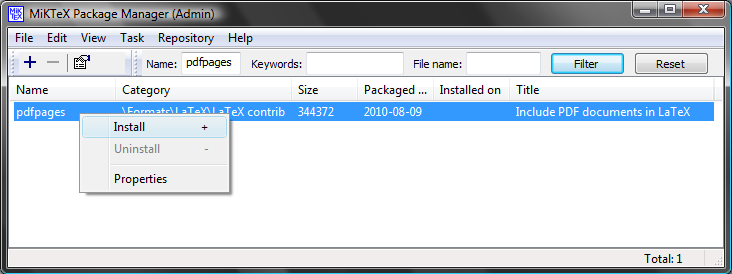
\includegraphics[width = 12cm]{figures/pakiety.png}
		\caption{Instalacja dodatkowych pakietów}
		\label{fig:pakiety}
	\end{center}
\end{figure}

\section{Pakiet Bib\TeX}
\label{sec:tresc:bibtex}

Pakiet Bib\TeX służy do zarządzania bibliografią. Pozycje bibliograficzne zapisywane są w plikach tekstowych z rozszerzeniem $.bib$, a następnie wywołanie poleceniem $\backslash cite$. Pliki bib muszą mieć odpowiednią strukturę, którą można poznać na stronie \url{http://pl.wikipedia.org/wiki/BibTeX}, lub \url{http://en.wikipedia.org/wiki/BibTeX}.\\
Bibliografię tworzy się wywołując w dokumencie polecenie $\backslash bibliography$. Po skompilowaniu dokumentu zawierającego odwołania do bibliografii, należy skompilować bibliografię za pomocą osobnego przycisku, a następnie znów skompilować dokument. Kompiluje się jednak zawsze tylko z widoku głównego dokumentu. Bib\TeX sam uporządkuje bibliografię według podanego stylu, zamieszczając tylko te pozycje które zostały zacytowane. Styl bibliografii ustawiany jest poleceniem $\backslash bibliographystyle$ przed wywołaniem pierwszego cytowania. W tym dokumencie użyto stylu plplain.

%
\chapter{Podsumowanie}
\label{sec:podsumowanie}

W podsumowaniu należy pokrótce opisać sposoby i efekty realizacji celów pracy przedstawionych w rozdziale \ref{sec:wstep:cel}. Oprócz tego powinny siê tu znaleść wnioski wynikające z wyników pracy, oraz dalsze kierunki rozwoju zagadnienia.

\end{lstlisting}

\section{Wzory matematyczne w \LaTeX}
\label{sec:tresc:wzory}

Przykładowy wzór: odwrotna transformata Fouriera:

\begin{itemize}
\item Ciągła:

\begin{equation}
 f(x) = \mathcal{F}^{-1}\{\hat{f}(\xi)\} = \int\limits_{-\infty}^{\infty}\hat{f}(\xi)e^{2\pi ix\xi}dx
 \label{eq:f2}
\end{equation}

\item Dyskretna:

\begin{equation}
 f(n) = \frac{1}{N}\sum\limits_{k = 0}^{N-1}F_{DFT}(k)e^{j \frac{2\pi}{N}nk}dx
 \label{eq:f4}
\end{equation}

\end{itemize}

Przykładowa macierz: elementarna macierz obrotu punktu wokół osi $x$ o kąt $\alpha$:

$$RotX(\alpha) = \left[ \begin{array}{c c c} 
1 & 0 & 0 \\
0 & cos(\alpha) & -sin(\alpha) \\ 
0 & sin(\alpha) & cos(\alpha)
\end{array} \right] $$

\section{Tabele}
\label{sec:tresc:tab}

Tabela \ref{tab1} zawiera przykładowe wyniki dwóch sprawdzianów.

\begin{table}[h]
	\begin{center}
	\caption{Przykladowa tabela}
	\label{tab1}
	\begin{tabular}{|c|c|c|c|}
		\hline
		Lp.& nr indeksu & \multicolumn{2}{|c|}{kolokwium}\\ \cline{3-4}
		   &            & I   & II \\ \hline
		1  & 32453      & 4,0  & 5,0\\
		2  & 42546      & 3,5  & 4,0\\
		3  & 32546      & 2,0  & 3,0\\ \hline
	\end{tabular}
	\end{center}
\end{table}

\section{Rysunki}
\label{sec:tresc:rys}

Rysunek \ref{fig:rys1} zawiera logo Politechniki Poznañskiej.\\

\begin{figure}[h]
	\begin{center}
		
\includegraphics[height = 3cm]{figures/template/logo-pp}
		\caption[Logo Politechniki Poznañskiej]{Logo Politechniki Poznañskiej; uwaga: w podpisach rysunków nie ma kropek na koñcu zdania; jeżeli zdañ jest więcej należy oddzielać je średnikami i zaczynać z małej litery}

		\label{fig:rys1}
	\end{center}
\end{figure}

\section{Dodawanie pakietów}
\label{sec:tresc:pakiety}

W przypadku użycia pakietu MiKTeX, aby zainstalować dodatkowe pakiety należy włączyć {\itshape Package Manager}, w katalogu {\itshape Maintenance (Admin)}. Następnie w pole {\itshape Name} wpisać nazwę brakującego pakietu i nacisnąć przycisk {\itshape Filter}. Nazwę wybranego pakietu należy kliknąć prawym przyciskiem myszy i nacisnąć {\itshape Install}, jak na rysunku \ref{fig:pakiety}.

\begin{figure}[h]
	\begin{center}
		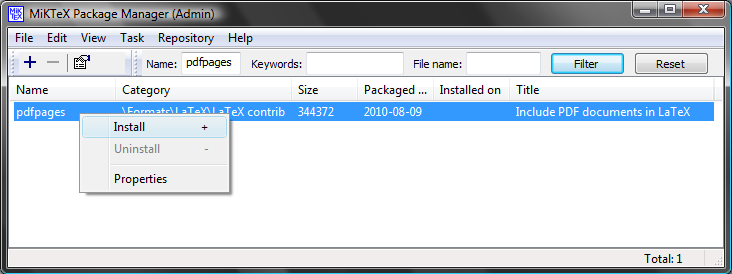
\includegraphics[width = 12cm]{figures/pakiety.png}
		\caption{Instalacja dodatkowych pakietów}
		\label{fig:pakiety}
	\end{center}
\end{figure}

\section{Pakiet Bib\TeX}
\label{sec:tresc:bibtex}

Pakiet Bib\TeX służy do zarządzania bibliografią. Pozycje bibliograficzne zapisywane są w plikach tekstowych z rozszerzeniem $.bib$, a następnie wywołanie poleceniem $\backslash cite$. Pliki bib muszą mieć odpowiednią strukturę, którą można poznać na stronie \url{http://pl.wikipedia.org/wiki/BibTeX}, lub \url{http://en.wikipedia.org/wiki/BibTeX}.\\
Bibliografię tworzy się wywołując w dokumencie polecenie $\backslash bibliography$. Po skompilowaniu dokumentu zawierającego odwołania do bibliografii, należy skompilować bibliografię za pomocą osobnego przycisku, a następnie znów skompilować dokument. Kompiluje się jednak zawsze tylko z widoku głównego dokumentu. Bib\TeX sam uporządkuje bibliografię według podanego stylu, zamieszczając tylko te pozycje które zostały zacytowane. Styl bibliografii ustawiany jest poleceniem $\backslash bibliographystyle$ przed wywołaniem pierwszego cytowania. W tym dokumencie użyto stylu plplain.

%
\chapter{Podsumowanie}
\label{sec:podsumowanie}

W podsumowaniu należy pokrótce opisać sposoby i efekty realizacji celów pracy przedstawionych w rozdziale \ref{sec:wstep:cel}. Oprócz tego powinny siê tu znaleść wnioski wynikające z wyników pracy, oraz dalsze kierunki rozwoju zagadnienia.

\end{lstlisting}

\section{Wzory matematyczne w \LaTeX}
\label{sec:tresc:wzory}

Przykładowy wzór: odwrotna transformata Fouriera:

\begin{itemize}
\item Ciągła:

\begin{equation}
 f(x) = \mathcal{F}^{-1}\{\hat{f}(\xi)\} = \int\limits_{-\infty}^{\infty}\hat{f}(\xi)e^{2\pi ix\xi}dx
 \label{eq:f2}
\end{equation}

\item Dyskretna:

\begin{equation}
 f(n) = \frac{1}{N}\sum\limits_{k = 0}^{N-1}F_{DFT}(k)e^{j \frac{2\pi}{N}nk}dx
 \label{eq:f4}
\end{equation}

\end{itemize}

Przykładowa macierz: elementarna macierz obrotu punktu wokół osi $x$ o kąt $\alpha$:

$$RotX(\alpha) = \left[ \begin{array}{c c c} 
1 & 0 & 0 \\
0 & cos(\alpha) & -sin(\alpha) \\ 
0 & sin(\alpha) & cos(\alpha)
\end{array} \right] $$

\section{Tabele}
\label{sec:tresc:tab}

Tabela \ref{tab1} zawiera przykładowe wyniki dwóch sprawdzianów.

\begin{table}[h]
	\begin{center}
	\caption{Przykladowa tabela}
	\label{tab1}
	\begin{tabular}{|c|c|c|c|}
		\hline
		Lp.& nr indeksu & \multicolumn{2}{|c|}{kolokwium}\\ \cline{3-4}
		   &            & I   & II \\ \hline
		1  & 32453      & 4,0  & 5,0\\
		2  & 42546      & 3,5  & 4,0\\
		3  & 32546      & 2,0  & 3,0\\ \hline
	\end{tabular}
	\end{center}
\end{table}

\section{Rysunki}
\label{sec:tresc:rys}

Rysunek \ref{fig:rys1} zawiera logo Politechniki Poznañskiej.\\

\begin{figure}[h]
	\begin{center}
		
\includegraphics[height = 3cm]{figures/template/logo-pp}
		\caption[Logo Politechniki Poznañskiej]{Logo Politechniki Poznañskiej; uwaga: w podpisach rysunków nie ma kropek na koñcu zdania; jeżeli zdañ jest więcej należy oddzielać je średnikami i zaczynać z małej litery}

		\label{fig:rys1}
	\end{center}
\end{figure}

\section{Dodawanie pakietów}
\label{sec:tresc:pakiety}

W przypadku użycia pakietu MiKTeX, aby zainstalować dodatkowe pakiety należy włączyć {\itshape Package Manager}, w katalogu {\itshape Maintenance (Admin)}. Następnie w pole {\itshape Name} wpisać nazwę brakującego pakietu i nacisnąć przycisk {\itshape Filter}. Nazwę wybranego pakietu należy kliknąć prawym przyciskiem myszy i nacisnąć {\itshape Install}, jak na rysunku \ref{fig:pakiety}.

\begin{figure}[h]
	\begin{center}
		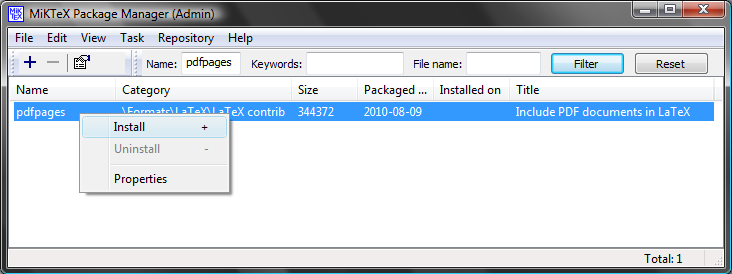
\includegraphics[width = 12cm]{figures/pakiety.png}
		\caption{Instalacja dodatkowych pakietów}
		\label{fig:pakiety}
	\end{center}
\end{figure}

\section{Pakiet Bib\TeX}
\label{sec:tresc:bibtex}

Pakiet Bib\TeX służy do zarządzania bibliografią. Pozycje bibliograficzne zapisywane są w plikach tekstowych z rozszerzeniem $.bib$, a następnie wywołanie poleceniem $\backslash cite$. Pliki bib muszą mieć odpowiednią strukturę, którą można poznać na stronie \url{http://pl.wikipedia.org/wiki/BibTeX}, lub \url{http://en.wikipedia.org/wiki/BibTeX}.\\
Bibliografię tworzy się wywołując w dokumencie polecenie $\backslash bibliography$. Po skompilowaniu dokumentu zawierającego odwołania do bibliografii, należy skompilować bibliografię za pomocą osobnego przycisku, a następnie znów skompilować dokument. Kompiluje się jednak zawsze tylko z widoku głównego dokumentu. Bib\TeX sam uporządkuje bibliografię według podanego stylu, zamieszczając tylko te pozycje które zostały zacytowane. Styl bibliografii ustawiany jest poleceniem $\backslash bibliographystyle$ przed wywołaniem pierwszego cytowania. W tym dokumencie użyto stylu plplain.

% konfiguracja listingów
\lstset{language=Verilog,
    numbers=left,
    frame=single,
    breaklines=true,
    captionpos=t,
    numberfirstline=false}

\chapter{Logika Programowalna}
\label{sec:logika}
\textit{Autor: Tomasz Kostur}

%==============================================================================
\section{Struktura projektowania komponentów logiki programowalnej}
\label{sec:logika:struktura}

Środowisko Xillinx Vivado udostępnia w swoim API jako górną warstwę abstrakcji
edytor schematu blokowego.Schemat blokowy jest czytelnym sposobem na szybkie
zapoznanie się z projektem i jego komponentami.
Komponentami schematu blokowego są bloczki IP (Intelectual Property).
W skład bloczków IP wchodzą przede wszystkim urządzenia dostępne poprzez magistralę
AXI w jej trzech rodzajach (AXI-lite, AXI-full, AXI-stream), bloczek symbolizujący processor
\textit{Zynq7 Processing System}, oraz specjalne bloczki generujące sygnały reset
lub obsługujące wybraną część magistrali AXI \textit{AXI Interconnect}.
Rysunek \ref{fig:block} przedstawia docelowy schemat blokowy projektu.

\begin{figure}[h]
    \begin{center}

    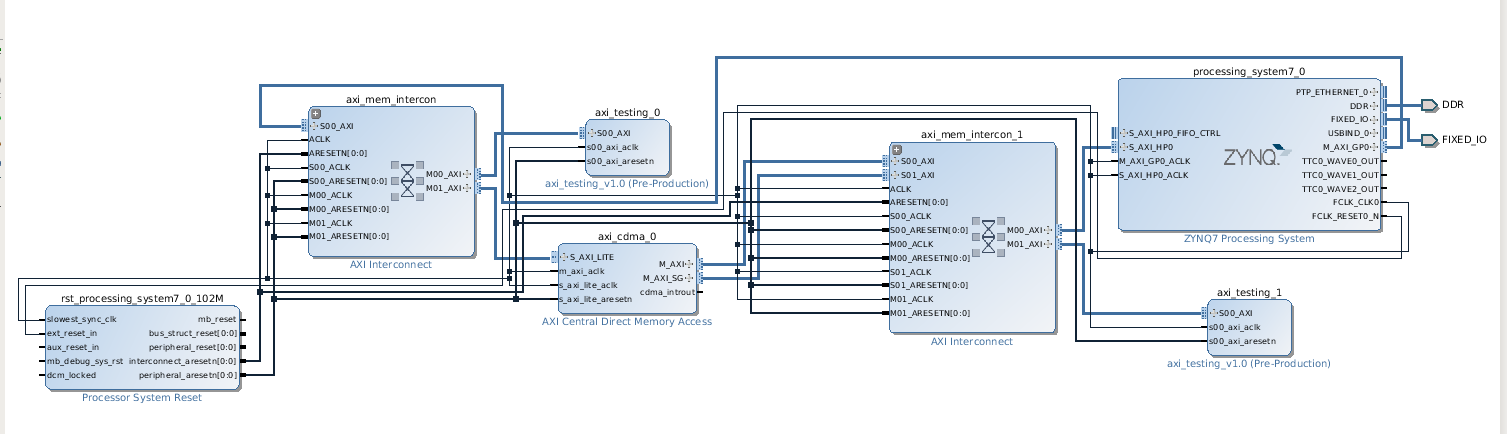
\includegraphics[height = 5cm]{figures/axi_matching_block_design.png}
    \caption["Wypłaszczanie macierzy"]{Docelowy schemat połączeń komponentów w block design}
    \label{fig:block}

    \end{center}
\end{figure}




Docelowy schemat blokowy przedstawia dwie alternatywne instancje jednego ze zbudowanych
urządzeń IP.
(moduł porównujący opisany w rozdziale \ref{sec:logika:matchowanie} lub moduł zwracający 
 dysparycje opisany w rozdziale \ref{sec:logika:dysparycja})
Jedna z instancji jest dostępna jako element podlegający bloczkowi procesora,
dróga jest dostępna jako slave bloczka \textit{AXI Central DMA}
(opisany w rozdziale \ref{sec:logika:cdma}).
Połączenia pomiędzy
bloczkami master-slave są realizowane poprzez bloczek pośredniczący \textit{AXI Interconnect}.
Bloczek \textit{AXI Interconnect} realizuje połączenia magistrali na zasadzie:
każdy podłączony układ master ma dostęp do każdego podłączonego układu slave.

Podsumowując schemat połączeń:
\begin{itemize}
\item Bloczek symbolizujący procesor jest masterem dla bloczków \textit{AXI Central Dma} oraz
jednej z instancji bloczka przetwarzającego. Procesor może w ten sposób zapisywać i odczytywać dane
z bloczka przetwarzającego oraz zapisywać i odczytywać rejestry konfiguracyjne CDMA.
\item Bloczek \textit{AXI Centrall Dma} jest masterem dla drugiej z instancji bloczka
przetwarzającego, oraz masterem dla portu procesora \textit{AXI High Performance}.
Dzięki połączeniu do dodatkowego portu slave procesora Centrall DMA może zapisywać
i odczytywać dane z pamięci RAM procesora.
\end{itemize}

%******************************************************************************

\section{Moduł AXI Centrall DMA}
\label{sec:logika:cdma}

Moduł DMA (Direct Memory Access) jest urządzeniem przenoszącym dane z jednego miejsca w pamięci
do drugiego.
Dzięki DMA można znacznie odciążyć procesor z wielu zadań kopiowania dużych ilości
danych w pamięci. Docelowym zadaniem DMA w aplikacji jest całkowite zautomatyzowanie
przesyłania danych z pamięci ram procesora do układu fpga i z powrotem.
W środowisku Vivado mamy do dyspozycji dwie wersje tego urządzenia


\begin {itemize}
\item \textit{AXI DMA} łączące urządzenia \textit{memory mapped}, z
urządzeniami z magistralą \textit{AXI stream}. Bloczek potrafiprzesyłać dane oraz
konwertować jeden typ danych na drugi.
\item \textit{AXI Central Dma} wersja urządzenia służąca do przekazywania danych
pomiędzy podległymi mu urządzeniami z magistralą mapowaną jako pamięć
(\textit{AXI-lite, AXI-full, AXI High Performance} procesora)
\end{itemize}

W aplikacji użyty został \textit{AXI Central Dma}

Dwa główne tryby pracy Central DMA to \textit{simple mode} oraz \textit{scattes gatter}

\subsection{Central DMA - simple mode}
\label{sec:logika:dma:simple}

Zaprogramowanie zadania przeniesienia danych przez DMA sprowadza się do zapisania w pamięci fizycznej
odpowiednich rejestrów konfigurujących CDMA. Adres rejestru startowego jest automatycznie
generowany przez Vivado. Kolejne rejestry konfiguracyjne następują po sobie zgodnie
z 32-bitowym adresowaniem pamięci (a więc co 4 bajty danych).


\begin{table}[h]
    \begin{center}
    \caption{Tabela niezbędnych rejestrów używanych w CDMA}
    \label{tab:cdmareg}

    \begin{tabularx}{\textwidth}{|c|c|X|}
        \hline
        offset & nazwa rejestru & wyjaśnienie \\ \hline

        0x00   & CDMACR         & Central DMA Controll Register.
                                    jest odpowiedzialny za wybór trubu pracy CDMA,
                                    ustawianie systemu przerwań, resetowanie urządzenia \\ \hline

        0x04  & CDMASR          & Central DMA Status Register. Odpowiedzialny za rozpoznawanie
                               błędów, zaistniałych przerwań, statusu transferu. \\ \hline

        0x08 & CURDESC\_PNTR & Adres pamięci fizycznej aktualnie przetwarzanego deskryptora w \textit{,,scatter gather''} \\ \hline

        0x10 & TAILDESC\_PNTR & Adres pamięci fizycznej odtatniego deskryptora w \textit{,,scatter gather''}. Zapisanie wartości tego
                                rejestru rozpoczyna serie transferów, osiągnięcie wartości TAILDESC\_PTNR przez CURDESC\_PNTR kończy
                                serie transferów i ustawia bit w CDMASR sygnalizujący stan \textit{,,iddle''} \\ \hline

        0x18  & SA              & Source Address. Adres od którego rozpoczyna się seria danych
                                  do transferu w \textit{,,simple mode''} \\ \hline

        0x20   & DA             &  Destination Address. Początkowy adres miejsca w pamięci do którego
                                   dana mają zostać przekopiowane w \textit{,,simple mode''} \\ \hline

        0x28 &        BTT       &  Bytes to Transfer. Liczba bitów jaka ma być przekopiowana w \textit{,,simple mode''}. \\ \hline
    \end{tabularx}
\end{center}
\end{table}


W tableli \ref{tab:cdmareg} przedstawiono poszczególne rejestry CDMA oraz ich krótkie
wyjaśnienie. Kolumna \textit{offset} oznacza odległość w bajtach od początkowego rejestru
CDMA. Dla CDMA \textit{simple mode} konieczne jest zapisanie rejestrów: kontrolnego
\textit{CDMACR}, statusu \textit{CDMASR}, adresu danych do przekopiowania \textit{,,SA''},
adresu docelowego \textit{,,DA''}, ilości bajtów do przekopiowania \textit{,,RTT''}

Po zapisaniu wszystkich rejestrów następuje start pojedyńczego transferu.

\subsection{Central DMA - scatter gather}
\label{sec:logika::dma:sg}

Podczas gdy jest niezbędnym wykonanie wielu transferów o różnych adresach
source i destinadion, warto jest skorzystać z opcji \textit{,,scatter gather''}.
Opcja ta umożliwia korzystanie ze specjalne struktury zapisywanej w pamięci,
najczęściej ramu procesora,
definiującej kolejne zadania CDMA.

Zadania CDMA w opcji \textit{,,scatter gather''} są definiowane przez deskryptory.
Deskryptory zawierają dane adresów początkowych transferów, docelowych, oraz liczbę bitów,
podobnie jak do jest w \textit{,,simple mode''}.
Podanto każdy deskryptor zawiera początkowy adres następnego deskryptora, oraz
rejestr statusu wykonania zadania. Struktura pojedyńczego deskryptora
zadania CDMA przedstawiona jest w tabeli \ref{tab:cdmadesc}.

\begin{table}[h]
    \begin{center}
    \label{tab:cdmadesc}
    \caption{Tabela struktury pojedyńczego deskryptora zadania CDMA}
    \begin{tabularx}{\textwidth}{|c|c|X|}
        \hline
        offset & nazwa rejestru & wyjaśnienie \\ \hline \hline
        0x00 & NEXTDESC\_PNTR & Adres fizycznej pamięci następnego deskryptora \\ \hline
        0x08 & SA & Adres fizyczny początku danych do przekopiowania (\textit{,, Source Address''}) \\ \hline
        0x10 & DA & Adres fizyczny miejsce docelowego danych (\textit{,, Destination Address''}) \\ \hline
        0x18 & CONTROL & Ilość bajtów do przekopiowania \\ \hline
        0x1C & STATUS & Resestr zapisywany przez CDMA, oznaczający status wykonania zadania
                        definiowanego przez deskryptor. Morze wskazywać na poprawne wykonane
                        zadanie lub wystąpienie błędu. \\ \hline
    \end{tabularx}
    \end{center}
\end{table}


Przykładowa implementacja struktury deskryptorów w pamięci fizycznej została przedstawiona
na listingu \ref{lst:tcl}.

%******************************************************************************

\section{Działanie modułu porównującego}
\label{sec:logika:matchowanie}

Pierwszym modułem jaki wykonano w języku verilog, jest moduł porównujący ze sobą
dwie maski obrazu. Wielkość maski jest podawana w sparametryzowany sposób, jako
argument syntezy modułu. (Po zakończeniu procesu syntezy i wygenerowaniu bitstream-u)
    nie ma możliwości zmiany rozmiaru maski. 


Docelowy interfejs AXI-full udostępnia wymianę danych pomiędzy procesorem, a logiką
programowalną na zasadzie zapisywania i odczytywania do pamięci. W związku z tym
wszelkie abrstrkcje przekazywane jako argumenty do dalszego przetwarzania w module
muszą zostać przekazane jako jednowymiarowy wektor danych. Odpowiednie argumenty
mają więc odpowiedni przedział adresów.
W napisanych urządzeniach przyjęto standardową konwencje zapisywania macierzy
od prawej do lewej z góry do dołu. Kolejne macierze, lub dodatkowe przekazywane
dane następują bezpośrednio po sobie.
Na rysunku \ref{fig:wyplaszczanie} przedstawiono sposób "wypłaszczania" macierzy.

\begin{figure}[h]
    \begin{center}

    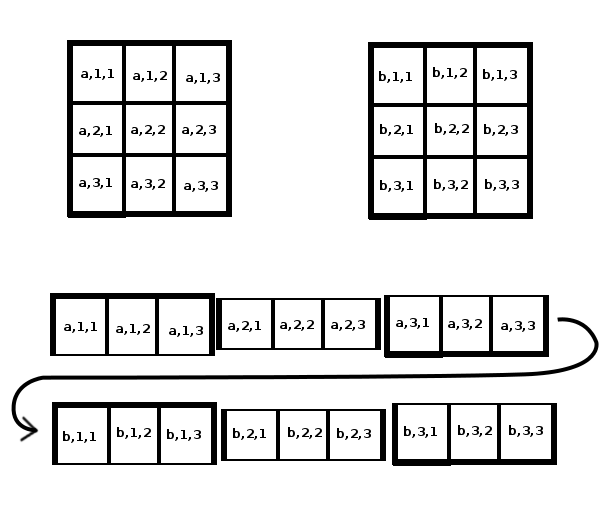
\includegraphics[height = 8cm]{figures/flattern_matrixes.png}
    \caption["Wypłaszczanie macierzy"]{Sposób w jaki abstrakcja macierzy zostaje
        zapisana do pamięci modułu, jako jednowymiarowy wektor danych}
    \label{fig:wyplaszczanie}

    \end{center}
\end{figure}

Listing \ref{lst:flattern} przedstawia fragment test-bench-u przypisujący
z pojedynczego wektora danych \textit{"data vector"} do jakiego mamy dostęp poprzez
interfejs AXI-full do etykiet oznaczających abstrakcje macierzy w celu dalszego
ich przetwarzania jako argumenty zadania. Takie oznaczenie jest niezbędne dla
czytelności kodu i realizacji zadania, nie jest natomiast konieczne oznaczenie
macierzy jako tablicy dwuwymiarowej. W dalszej części kodu macierze są przetwarzane
jako dwa pojedyncze wektory danych.
   

\begin{lstlisting}[caption={fragment test bench w języku verilog przedstawiający
    sposób przypisania},label={lst:flattern}]

parameter MASK_SIZE = 3;
parameter matrix_cells = MASK_SIZE * MASK_SIZE;

    wire [8-1 : 0] mask_left [matrix_cells -1 : 0];
    wire [8-1 : 0] mask_right [matrix_cells -1 : 0];
    genvar i;
    generate
	for (i=0 ; i<matrix_cells ; i=i+1)begin
		assign mask_left[i] = data_vector[i];
		assign mask_right[i] = data_vector[i + matrix_cells];
	end
    endgenerate

\end{lstlisting}


Sposób w jaki porównywane są macierze to odjęcie od siebie, z wartością bezwzględną
odpowiadających sobie pikseli, a następnie zsumowanie wszystkich różnic
(równanie \ref{eq:match}).
Im mniejszy wynik tym lepsze dopasowanie macierzy.

\begin{equation}
E=\sum_{i=0}^{matrix\_cells}|M_{1}[i]-M_{2}[i] |
\label{eq:match}
\end{equation}

Porównywanie zrealizowano na układzie kombinacyjnym dlatego równolegle w czasie
dokonują się wszystkie odejmowania. Suma wszystkich odejmowań jest natomiast
zrealizowana następująco:

\begin{itemize}

\item pierwszy rejestr wektora \textit{"summation\_steps"} jest sumą pierwszego
odejmowania z drugim.

\item każdy następny element wektora \textit{"summation\_steps"} jest sumą poprzedniego
elementu tego wektora z następnym odejmowaniem.

\item ilość elementów wektora \textit{"summation\_steps"} jest o jeden mniejsza
niż ilość elementów wektora reprezentującego macierz. Ostatni element wektora
jest sumą wszystkich odejmowań

\end{itemize}

Rysunek \ref{fig:matching} obrazuje ułożenie poszczególnych etykiet połączeń
wektora \textit{"summation\_steps"} w układzie.

\begin{figure}[h]
    \begin{center}

    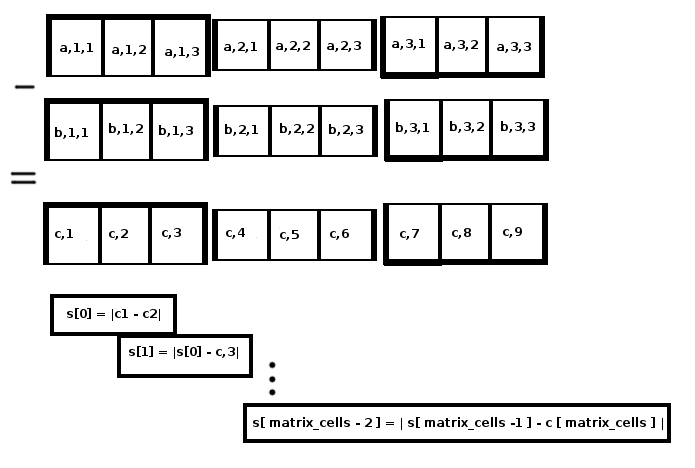
\includegraphics[height = 8cm]{figures/combinational_matching.png}
    \caption["Dopasowywanie macierzy"]{Sposób w jaki ułożone są etykiety
    wektorów połączeń realizujące dopasowywanie dwóch macierzy}
    \label{fig:matching}

    \end{center}
\end{figure}

Listing \ref{lst:matching} przedstawia realizację zadania w języku Verilog.
Odejmowanie z wartością bezwzględną zostało zrealizowane przez multiplekser
dołączony do każdego odejmowania. Multiplekser definiuje kolejność odejmowania
od siebie zmiennych, tak aby zawsze mniejsza była odejmowana od większej.

\begin{lstlisting}[caption={Realizacja zadania match-owania macierzy w języku Verilog},
label={lst:match}]
//combinational per element substraction (diffrence_per_element is result)
wire [8-1 : 0] diffrence_per_element [matrix_cells -1 : 0];
genvar i;
generate
	for ( i=0; i<matrix_cells; i = i+1)begin
		assign diffrence_per_element[i] = (mask_left[i]>mask_right[i])? mask_left[i] - mask_right[i] : mask_right[i] - mask_left[i];
	end
endgenerate
//combinational sum

parameter summation_steps_bits = 11 ;// 11 bits for max MAX_SIZE = 15
wire [summation_steps_bits -1 : 0] summation_steps [matrix_cells-2 : 0];
generate
	assign summation_steps[0] = diffrence_per_element[0] + diffrence_per_element[1];
	for (i=0; i<matrix_cells-2; i=i+1) begin
		assign summation_steps[i+1] = summation_steps[i] + diffrence_per_element[i+2];
	end
endgenerate
wire [summation_steps_bits-1 : 0] diffrence_sum;
assign diffrence_sum = summation_steps[matrix_cells - 2];

\end{lstlisting}

Wynikiem jest zmienna \textit{"diffrence\_sum"}.
Kody z listingów tego rozdziału są załączone w kod generowany przez Vivado.
Dalsze przypisania do magistrali
AXI-full są wytłumaczone w rozdziale \ref{sec:logika:magistrala:full}


%*******************************************************************************


\section{Działanie modułu zwracającego dysparycje}
\label{sec:logika:dysparycja}

Kolejnym krokiem rozszerzającym jest wykonanie modułu zwracającego wartość dysparycji.

Z powodu na większą złożoność, aby umożliwić sprawne debugowanie kod realizujący
zadanie spakowano w dyrektywę \textit{"module"} języka Verilog, zamiast załączać 
go w całości do kodu magistrali AXI-full tak jak to zrobiono w podrozdziale \ref{sec:logika:matchowanie}

Ograniczeniem dyrektywy \textit{"module"} jest brak możliwości przekazywania
argumentów jako tablic wielowymiarowych lub wektorów. Jedyną możliwością przekazywania
argumentów są pojedyncze wektory bitów(listing \ref{lst:callmod}). Za każdym razem więc chcąc przekazać
dane do modułu należy je "wypłaszczyć" do takich wektorów(listing \ref{lst:flat2bits}),
wewnątrz modułu należy je z powrotem oznaczyć etykietami połączeń jako tablice
lub odpowiednio inne typy danych (listing \ref{lst:bits2vec}).

\begin{lstlisting}[label={lst:callmod},
caption={wywoływanie kodu modułu "stereo\_solver" urządzenia w języku Verilog}]
stereo_solver #
(
	.MASK_SIZE(MASK_SIZE),
	.MATCH_WIDE(MATCH_WIDE),
	.POSITION_BITS(8)
)
solver_inst(
	.flattern_mask(flattern_mask),
	.flattern_match_array(flattern_match_array),
	.mask_position(mask_position),
	.match_position(match_position),
	.DISSPARITION(dissparition)
);

\end{lstlisting}

\begin{lstlisting}[caption={oznaczenie części wektora danych "data\_vector"
    jako poszczególne zmienne oraz
    wypłaczczanie wektorów danych do wektorów bitów},label={lst:flat2bits}]

wire [8-1 : 0] mask [matrix_cells-1 : 0];
wire [8-1 : 0] match_array [MASK_SIZE*MATCH_WIDE-1 : 0];

generate
	for(i=0; i<matrix_cells; i=i+1)begin
		assign mask[i] = data_vector[i][8-1 : 0];
	end
	for(i=0; i<MASK_SIZE*MATCH_WIDE; i=i+1)begin
		assign match_array[i] = data_vector[i+matrix_cells][8-1 : 0];
	end
	for(i=0; i<MASK_SIZE*MASK_SIZE; i=i+1)begin
		assign flattern_mask[i*8 +: 8] = mask[i];
	end
        
	for(i=0; i<MASK_SIZE*MATCH_WIDE; i=i+1)begin
		assign flattern_match_array[i*8 +: 8] = match_array [i];
	end
	assign mask_position = data_vector [matrix_cells + MASK_SIZE*MATCH_WIDE];
	assign match_position = data_vector[matrix_cells + MASK_SIZE*MATCH_WIDE+1];

endgenerate
\end{lstlisting}

\begin{lstlisting}[label={lst:bits2vec},
    caption={odzyskiwanie struktury wektorów danych z wektora bitów}]

wire  [MASK_SIZE*MASK_SIZE-1 : 0] maskA [MATRIX_CELLS-1 : 0];
wire  [MASK_SIZE*MASK_SIZE-1 : 0] maskB [MATRIX_CELLS-1 : 0];
//wypelnianie tablicy z wektora bitow
genvar i;
generate
	for(i=0; i<MATRIX_CELLS; i=i+1) begin
		assign maskA[i] = flattern_maskA [i*8 +: 8];
		assign maskB[i] = flattern_maskB [i*8 +: 8];
	end
endgenerate

\end{lstlisting}

\begin{lstlisting}[label={lst:matchdec},
caption={deklaracja modułu realizującego dopasowywanie macierzy}]

module matcher #
(
	parameter MASK_SIZE = 3,
	parameter MATRIX_CELLS = 9,
	parameter SUMMATION_STEPS_BITS = 11 //11 for max MASK_SIZE = 15;
)
(
	input wire  [8*MATRIX_CELLS-1 : 0] flattern_maskA,
	input wire  [8*MATRIX_CELLS-1 : 0] flattern_maskB,
	output wire [SUMMATION_STEPS_BITS-1 : 0] match
);


\end{lstlisting}


Aby zachować wspomnianą wcześniej wygodę przy debugowaniu oraz pewność poprawnego działania
w dyrektywę \textit{"module"} spakowano również kod z dopasowywujący macierze
z podrozdziału \ref{sec:logika:matchowanie}. Deklaracja modułu jest widoczna na
listingu \ref{lst:matchdec}.

Zadania jakie więc należy wykonać w module zwracającym dysparycję to:

\begin{itemize}
\item Pobranie maski dopasowania.
\item Pobranie przestrzeni dopasowania macierzy.
\item Wygenerowanie wektora porównań maski z przestrzenią porównań.
\item Wybór najlepszego dopasowania z wektora porównań.
\item Obliczenie dysparycji na podstawie danych: położenia maski,
    połorzenia przestrzeni porównań, numeru najlepszego porównania.
\end{itemize}

Wektor porównań został stworzony dzięki dyrektywie \textit{"generate"}
która w sparametryzowany sposób umożliwia wygenerowanie odpowiedniej ilości
modółów porównujących do syntezy. Wygenerowanie wektora porównań z użyciem
modułu porównującego (deklaracja listing \ref{lst:matchdec}) przedstawione jest
na listingu \ref{lst:mathcvector}

\begin{lstlisting}[label={lst:matchdec},
caption={wygenerowywanie wektora porównań macierzy z przestrzenią porównań}]

genvar i,j,k;
parameter matches_vector_cells = MATCH_WIDE-(MASK_SIZE-1);
// deklaracja wektora kolejnych porownan
wire [13-1 : 0] matches_vector [matches_vector_cells-1 : 0];//13 od 255*25 = 6000 ponad wiec 2^13
// 13 bitow dla maksymalnej maski 5x5
generate
// petla generujaca kolejne wyniki porownan
    for(i=0; i<matches_vector_cells; i=i+1)begin
        wire [8-1 : 0] match_mask [MASK_SIZE-1 : 0][MASK_SIZE-1 : 0];
// petla wskazujaca wlasciwa maske do porownania z posrod pikseli przestrzeni porownan
        for(j=0; j<MASK_SIZE; j=j+1)begin
            for(k=0; k<MASK_SIZE; k=k+1)begin
                assign match_mask[j][k] = flattern_match_array[((k+i)*8+j*MATCH_WIDE*8)  +: 8];
	    end
        end
//wyplaszczanie maski do wektora bitow w celu przekazania do modulu porownujacego
	wire [8*mask_cells-1 : 0] flattern_match_mask;
	for (j=0; j<MASK_SIZE; j=j+1) begin
	    for(k=0; k<MASK_SIZE; k=k+1)begin
		assign flattern_match_mask[j*MASK_SIZE*8+k*8 +: 8] = match_mask[j][k];
	    end
	end
// przekazanie maski oraz maski wycietej z przestrzeni porownan do modulu porownujacego
        matcher # 
	(
	    .MATRIX_CELLS(mask_cells),
	    .SUMMATION_STEPS_BITS(11)
	)
	gen_matcher (
	    .flattern_maskA(flattern_mask),
	    .flattern_maskB(flattern_match_mask),
// wypelnienie odpowiedniej komorki wektora porownan
	    .match(matches_vector[i])
	);
    end
endgenerate

\end{lstlisting}

Aby stworzyć strukturę która w sparapetryzowany sposób wybierała najmniejszy z
pośród elementów wektora dopasowań, będąc układem kombinacyjnym postanowiono
użyć następującego sposobu.

\begin{itemize}

\item Stworzono wektor \textit{"sort\_vec"} którego początkowa część jest tożsama
z wektorem kolejnych porównań

\item każdy następny element wektora \textit{"sort\_vec"} jest minimalną wartością
z dwóch kolejno nastpujących po sobie komórek tego wektora. Dwie wykorzystane
komórki do porównań nie są już wykorzystywane w następnych porównaniach dlatego
podczas gdy krok inkrementacji komórki wpisywanej jest równy 1, to inkrementacja
numerów komórek do wyboru wynosi 2. Wyjaśnia to rysunek \ref{fig:combmin}.

\item W ten sposób po odpowiednio dużej ilości porównań końcowy element wektora
\textit{"sort\_vec"} będzie najmniejszą jego wartością. Każda część wektora
będąca początkiem pobierania do porównania dwóch wyników poprzednich porównań
jest nazywana w dalszej części "stopniem porównań".

\item kolejne stopnie porównań wektora mają wymiar malejącego ciągu geometrycznego
 o ilorazie $$ q=\frac{1}{2} $$ dlatego długość całego wektora i wynikająca z
 niej potrzebna ilość iteracji jest częścią całkowitą z sumy nieskończonego
 ciągu geometrycznego o pierwszym wyrazie równym długości wektora porównań.

\begin{equation}
sort\_vec\_cells =  \left[ \frac{matches\_vector\_cells}{1- \frac{1}{2} }  \right]
\label{eq:sortcells1}
\end{equation}

\item Jeśli dla ułatwienia tak dobrać wielkość maski i przestrzeni porównań aby
wektor porównań miał by wielkość równą jakiejś potęgi dwójki wówczas
mamy pewność, że wszystkie składniki ciągu są liczbami całkowitymi, a
długość wektora
\textit{sortvec} upraszczała by się do:

\begin{eqnarray}
\label{eq:sortcells2}
sort\_vec\_cells = \frac{matches\_vector\_cells}{1- \frac{1}{2} } - \frac{1/2}{1-\frac{1}{2}} \\
sort\_vec\_cells = matches\_vector\_cells * 2 - 1
\end{eqnarray}

\item dołączając równoległy wektor wypełniony kolejnymi liczbami i wykonując
na nim identyczne operacje przenosin wartości co w \textit{sort\_vec} na jego
końcy otrzymujemy numer (jego odległość od początku \textit{sort\_vec}) najlepszego dopasowania.

\end{itemize}

\begin{figure}[h]
    \begin{center}

    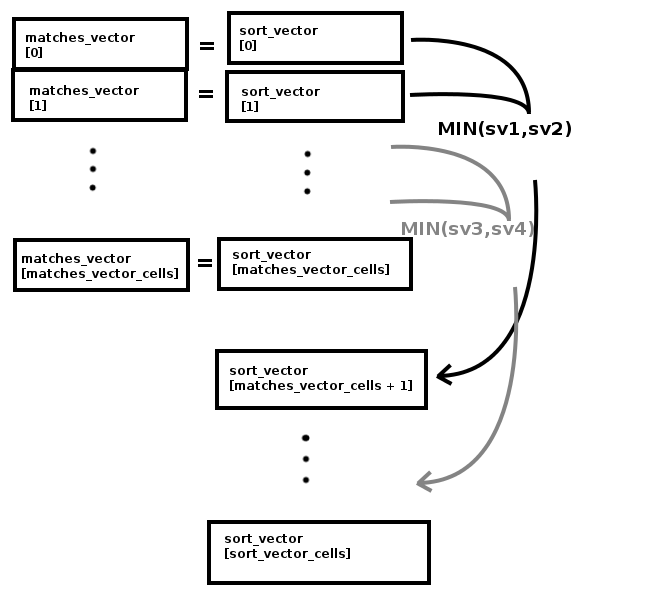
\includegraphics[height = 8cm]{figures/combinational_minimum.png}
    \caption["Minimum kombinacyjne"]{Sposób w jaki w całkowicie sekwęcyjny sposów
    uzyskano minimum z wektora}
    \label{fig:combmin}
    \end{center}
\end{figure}


Sposób w jaki zaimplementowano powyższy algorytm w języku Verilog przedstawiono na
listingu \ref{lst:sort}

\begin{lstlisting}[label={lst:sort},
caption={kombinacyjne wybieranie najmniejszego elementu wektora w języku Verilog}]

parameter sort_vec_cells = matches_vector_cells*2-1;
wire [8-1 : 0] sort_vec [sort_vec_cells-1 : 0];
wire [8-1 : 0] sort_vec_cell [sort_vec_cells-1 : 0];

generate
    for(i=0; i<matches_vector_cells; i=i+1)begin
        assign sort_vec[i] = matches_vector[i];
        assign sort_vec_cell[i] = i;
    end
    for(i=0; i<sort_vec_cells-1; i=i+2)begin
        localparam push_cell = i/2 + matches_vector_cells;
        assign sort_vec[push_cell] = (sort_vec[i] < sort_vec[i+1])? sort_vec[i] : sort_vec[i+1];
        assign sort_vec_cell[push_cell] = (sort_vec[i] < sort_vec[i+1])? sort_vec_cell[i] : sort_vec_cell[i+1];

    end
endgenerate

wire [8-1 : 0] min_of_vector;
wire [8-1 : 0] min_of_vector_cell;
assign min_of_vector = sort_vec [sort_vec_cells-1];
assign min_of_vector_cell = sort_vec_cell [sort_vec_cells-1];


\end{lstlisting}


%******************************************************************************
\section{Działanie generycznego kodu magistrali axi}
\label{sec:logika:magistrala}

W Xillinx Vivado tworzenie bloczka IP jest ułatwione dzięki automatycznemu generowaniu
części kodu logiki programowalnej implementującego bloczek z wybraną przez nas
ilością i rodzajem obsługiwanych magistrali AXI. Bloczek składa się z urządzenia
nadrzędnego zbierającego z sobie wszystkie urządzenia magistrali, oraz z plików poszczególnych
urządzeń. Ilość oraz rodzaj obsługiwanych urządzeń magistralowych jest dowolna.
W topowym module powinno unikać się wszelkich funkcjonalnych operacji logicznych.

Magistralami możliwymi do wyboru są:
\begin{itemize}
\item AXI-lite, charakteryzująca się ,,mało kosztownym'' rodzajem implementacji,
    przekazywane dane są tutaj poprzez generowane rejestry o nazwie \textit{,,slv\_regX''}
    gdzie X oznacza numer konkretnego rejestru. Magistrala nie jest szybka i słurzy przede wszystkim
    do przekazywania zmiennych konfiguracyjnych urządzeń.
\item AXI-stream. W przeciwieństwie do AXI-lite i AXI-full nie jest ona magistralą
    realizowaną na zasadzie modelowania pamięci. Axi-stream jest szybką magistralą
    umożliwiającą łączenie ze sobą pojedyńcze magistrale w szeregu na zasadzie
    master -> slave. Nie jest natomiast możliwe stworzenie sieci urządzeń działających na zasadzie
    klient server, z tego powodu m.in nie można podłączyć jej bezpośrednio do procesora.
    Możliwe jest konwertowanie wersji \textit{stream} do \textit{memory mapped}.
\item AXI-full jest szybszą wersją magistrali AXI-lite. Sposób w jaki odczytujemy przekazane
    do niej dane jest dokładniej przedstawiony w rozdziale \ref{sec:logika:magistrala:full}.
\end{itemize}

W aplikacji została użyta magistrala AXI-full ze względu na dostęp do przykładów,
  oraz możliwość bezpośredniego połączenia z bloczkiem \textit{,, Zynq Processing System 7''}.

\subsection{AXI full}
\label{sec:logika:magistrala:full}


Pośród wielu linijek wygenerowanego automatycznie, istnieje przykład implementacji
pamięci obsługiwanej przez AXI-full. Przykład ten posłurzył do stworzenia własnego
wektora danych przystosowanego do obsługi napisanych w rozdziałach
\ref{sec:logika:matchowanie} oraz \ref{sec:logika:dysparycja} modółów.

\begin{lstlisting}[label={lst:axifull},
    caption={fragment kodu łączący wygenerowany kod magistrali AXI-full z własnym modyłem}]
// sygnaly pozwolenia na zapis/odczyt do wektora danych
// data_vector	z magistrali
wire dvec_dren;
wire dvec_wren;
assign dvec_wren = axi_wready && S_AXI_WVALID;
assign dvec_rden = axi_arv_arr_flag;
// proces zapisania do wektora danych z magistrali
always @ (posedge S_AXI_ACLK) begin
    if (dvec_wren && S_AXI_WSTRB[0]) begin
        data_vector[mem_address] <= S_AXI_WDATA[8-1:0];
    end
end
// wyplaszczanie wektora danych do wektora bitow w celu przekazania
// danych do kolejnego modulu
wire [8-1 : 0] mask [matrix_cells-1 : 0];
wire [8-1 : 0] match_array [MASK_SIZE*MATCH_WIDE-1 : 0];
   
generate
    for(i=0; i<matrix_cells; i=i+1)begin
        assign mask[i] = data_vector[i][8-1 : 0];
    end
    for(i=0; i<MASK_SIZE*MATCH_WIDE; i=i+1)begin
        assign match_array[i] = data_vector[i+matrix_cells][8-1 : 0];
    end
    for(i=0; i<MASK_SIZE*MASK_SIZE; i=i+1)begin
    	assign flattern_mask[i*8 +: 8] = mask[i];
    end
 
    for(i=0; i<MASK_SIZE*MATCH_WIDE; i=i+1)begin
        assign flattern_match_array[i*8 +: 8] = match_array [i];
    end
    assign mask_position = data_vector [matrix_cells + MASK_SIZE*MATCH_WIDE];
    assign match_position = data_vector[matrix_cells + MASK_SIZE*MATCH_WIDE+1];

endgenerate
// odczyt z wektora do magistrali
always @ (posedge S_AXI_ACLK) begin
    data_vector[matrix_cells + MASK_SIZE*MATCH_WIDE + 2] <= dissparition;
end
// przekazanie danych do modlu
stereo_solver #
    (
    .MASK_SIZE(MASK_SIZE),
    .MATCH_WIDE(MATCH_WIDE),
    .POSITION_BITS(8)//(POSITION_BITS)
    )
    solver_inst(
    .flattern_mask(flattern_mask),
    .flattern_match_array(flattern_match_array),
    .mask_position(mask_position),
    .match_position(match_position),
    .DISSPARITION(dissparition)
    );
\end{lstlisting}

W uzyskanym rozwiązaniu zapisane dane pod odpowiednimi adresami są odpowiadającymi im
przekazywanymi zmiennymi. Cokolwiek natomiast zostaje odczytane z magistrali
jest wynikiem zwracany przez jeden z sekwęcyjnych modółów opisanych w rozdziałach
\ref{sec:logika:matchowanie} i \ref{sec:logika:dysparycja}.
Wynik jest zwracany na wszystkich adresach przestrzeni adresowej urządzenia AXI.


%******************************************************************************
\section{Narzędzia debugowania}
\label{sec:logika:debug}

Dużą częścią pracy jest opanowanie oraz napisanie kodów testowych.
W czasie tworzenia pracy opanowano 3 rodzaje debugowania są to odpowiednio:
\begin{itemize}
\item Bechawioralny symulator offline
\item Debugowanie poprzez interfejs JTAG działającej logiki na płytce rozwojowej
\item Debugowanie poprzez dostarczony program Xillinx Microprocessor Debugger
\end{itemize}
W niniejszym rozdziale zostały przedstawione najważniejsze informacje odnośnie używania
oraz ograniczeń poszczególnych sposobów weryfikacji programu.

\subsection{Behawioralny symulator offline}
\label{sec:logika:debug:simulation}

Jest to wstępny i najprostszy sposób debuggowania kodu logiki programowalnej.
Mając kod dowolnego modułu (dyrektywa \textit{"module"} w języku Veriog) tworzymy
testowy moduł nadrzędny generujący sygnały wejściowe do testowanego modułu.
Przykładowy "test bench" pokazany w listingu \ref{lst:testbench}.

\begin{lstlisting}[label={lst:testbench},
    caption={Przykładowy fragment kody Verilog użytego jako test bench}]

`timescale 1 ns / 1 ps

module stereo_solver_test_bench
    (
    );
// clock generation for test bench	
    reg clk = 0;

    always begin
    #5 clk = !clk;	
    end
	

    reg test_reg = 8;

    always @ (posedge clk) begin
        test_reg <= test_reg -1;
    end
endmodule
\end{lstlisting}

Jako wyjście z test bench-u otrzymujemy wektory przebiegów w czasie.
Rysunek \ref{fig:wave}) przedstawia interfejs jaki daje do dyspozycji Xillinx Vivado.
Dla testów przy użyciu symulatora język Verilog jak i VHDL udostępniają dodatkowe
funkcje nie mające wpływu na syntezę m.in
\begin{itemize}
\item dodatkowe stany logiczne: X-nieokreślony, Z-stan wysokiej impedancji
\item dyrektywa \textit{initial} wykonująca się tylko raz an początku wykonywania testu
\item dyrektywy opóźnień czasowych. Niezbędne przy modelowaniu sygnałów, np sygnału
zegarowego, lecz niemożliwe do syntezy bez połączenia z oscylatorem.
\end{itemize}

\begin{figure}[h]
    \begin{center}

    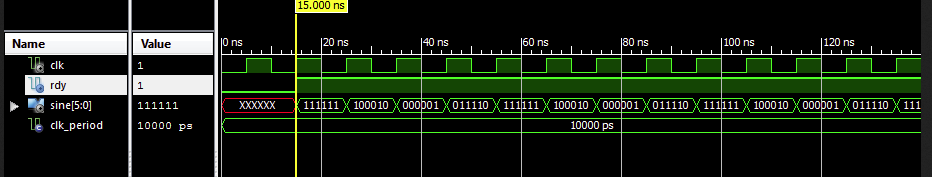
\includegraphics[height = 4cm]{figures/wave.png}
    \caption["Minimum kombinacyjne"]{Sposób w jaki w całkowicie sekwęcyjny sposów
    uzyskano minimum z wektora}
    \label{fig:combmin}
    \end{center}
\end{figure}


Mimo wielu zalet niestety taka symulacja offline nie zawsze jest całkowicie zgodna
z modułem stworzonym w procesie syntezy. Symulator używanego środowiska bywał
zawodny w następujących przypadkach:
\begin{itemize}
\item przypadków w których kluczowymi są różnice pomiędzy zmiennymi typu
\textit{reg} a \textit{wire} i odpowiednimi ich operatorami przypisania
\textit{=} oraz \textit{<=}
\item Przypisywanie stałych wartości do pewnych elementów wektora
\item Rożnych sposobów multipleksowania sygnałów
\end{itemize}

Zazwyczaj skutkowało to tym, że dobrze symulowany działający moduł, nie był możliwy
do syntezy lub implementacji.


\subsection{Debugowanie poprzez JTAG}
\label{sec:logika:debug:jtag}

Po zakończeniu procesu syntezy istnieje możliwość wskazania niektórych sygnałów
i stworzenia do nich wyprowadzeń (\textit{constraints}) do interfejsu JTAG.
Po powtórnym procesie syntezy, a następnie implementacji i załadowaniu bitstream-u,
wybieramy ilość próbek z jaką mają być pobrane zaznaczone sygnały i sygnały wyzwalania,
działające podobnie jak sygnały wyzwalania w oscyloskopie. Wyjściowym API
są tutaj przebiegi sygnałów w identycznym interfejsie jaki oferuje symulacja offline
\ref{fig:wave}

Słabą stroną tego sposobu jest fakt, że nawet przy wyłączonej opcji optymalizacji
syntezy, zsyntezowane sygnały i moduły mogą się znacznie różnić od tych jakie
zawarliśmy w kodzie. W procesie syntezy wiele kodu zostaje przekształconego lub
usuniętego.

\subsection{Xillinx Microprocessor Debug}
\label{sec:logika:debug:cmd}

Ostatecznym sposobem debugowania logiki programowalnej jest program XMD
(Xillinx Microprocessor Debugger). Jest to program udostępniający interfejs
konsolowy. Nieoceniony przy łączeniu logiki programowalnej z systemem operacyjnym.
Najbardziej przydatnymi funkcjami programu są:
\begin{itemize}
\item Możliwość programowania bitsream-u logiki programowalnej podczas pracy procesora
\item Możliwość sterowania procesorem poleceniami m.in \textit{rst con stop ...}
\item Możliwość swobodnego odczytywania rejestrów pamięci fizycznej, zarówno ram-u
jak i pamięci z przestrzeni addresów dostępnych dla processora magistrali AXI.
Komendy \textit{mrd} -czytanie z pamięci, oraz \textit{mwr} zapisywanie do pamięci
\end{itemize}

Program można dowolnie oskryptować używając składni \textit{tcl shell}.
Przykładowy skrypt programu używany do testowania DMA w listingu \ref{lst:tcl}


\lstset{language=tcl}
\begin{lstlisting}[label={lst:tcl},
    caption={fragment skryptu tcl wykorzystywany do testowania DMA}]
proc dma_sg_test {} {
#dane do przekopiowania
	mwr 0x10000000 10
	mwr 0x10000004 2
	mwr 0x10000008 3
	mwr 0x1000000C 4
# teraz deskryptory
	mwr 0x12000000 0x12000040
	mwr 0x12000008 0x10000000
	mwr 0x12000010 0x76000000
	mwr 0x12000018 4

	mwr 0x12000040 0x12000080
	mwr 0x12000048 0x10000004
	mwr 0x12000050 0x76000004
	mwr 0x12000058 4

#dwa zapisane do targetu to teraz odczytajmy
	mwr 0x12000080 0x12000000
	mwr 0x12000088 0x76000000
	mwr 0x12000090 0x11000000
	mwr 0x12000098 4

# ok no to teraz zapiszmy cdma controll register i inne
	mwr 0x4E200000 0x00010002
	mwr 0x4E200000 0x0001000A
	mwr 0x4E200008 0x12000000
	mwr 0x4E200010 0x12000080
#	mwr 0x4E200000 0x

#	mrd 0x11000000 3

}

proc d_reset {} {
	rst
	ps7_init
	ps7_post_config
	fpga -f design_1_wrapper.bit
	clear
	desc_clear
}

\end{lstlisting}


%******************************************************************************
\section{Napotkane problemy i możliwości optymalizacji}
\label{sec:logika:optymalizacja}


Poważnymi problemami jakie pojawiły się z związku z logiką programowalną są:

\begin{itemize}
\item Nawet w ,,czystym'' nie modyfikowanym kodzie magistrali AXI-full
    nie udawało się, przy użyciu CDMA przesłać więcej niż 4 bajty danych w obrębie
    jednego zadania kopiowania pamięci DMA.
\item W obrębie jednej tablicy desktyptorów zadań CDMA w \textit{,,statter gather''}
    mode nie udawało się użyć tego samego adresu fizycznego jako ,,source'' i ,,destination''.
    W przeciwnym razie moduł CDMA zawieszał się nie reagując na żadne komendy, w tym
    ,,soft reset''.
\end{itemize}

Jednym ze sposobów działania aplikacji jest:
\begin{itemize}
\item Zaalokowanie przy użyciu procesora pamięci fizycznej i wpisanie do nich
    prawego i lewego obrazka.
\item stworzenia tablicy deskryptorów CDMA oraz uruchomienie CDMA
\item odczytanie wyniku w postaci całego obrazu dysparycji, obliczonego w logice programowalnej i
    przeniesionego do ram-u procesora za pomocą CDMA
\end{itemize}

W ten sposób niemal całkowicie odciążony procesor, miał by zwolniony czas
na programy działające w systemie, komunikacje itp. Jednak konsekwencją wymienionych niedoskonałości
jest konieczność resetowania zadanej tablicy deskryptorów zanim wystąpi przypadek
w którym jeden z \textit{,,destination address''} staje się \textit{,,source address''}.
W programie problem ten rozwiązano odpowiednio dzieląc pełną tablicę deskryptorów
i zadając ją segmentami do CDMA w taki sposób aby omawiany błąd nigdy nie wystąpił.
Nie jest to jednak rozwiązanie optymalne ponieważ koniecznym jest ciągłe monitorowanie
rejestru statusu CDMA.

Być może innym rozwiązaniem tego problemu mogło by się okazać taka implementacja
urządzenia AXI w której dane wejściowe mogą być odczytane, a wynik podawany jest jako
odrębny dares przestrzeni adresowej modułu IP.

Konsekwencją błędu w którym poprzez jedno zadanie CDMA jesteśmy w stanie przesłać jedynie 4 bajty,
    co w stworzonej implementacji oznacza zaledwie jeden piksel z obrazu danych wejściowych,
    jest po raz kolejny spowolnienie przepływu danych, ale też bardzo duże wymagane
    rozmiary pamięci na dane oraz deskryptory.

Każdy piksel jest przechowywany jako zmienna 32-bitowa co przy dwóch obrazach
o rozdzielczości 800x600 daje 
\begin{equation}
3*800*600*4=5.76 Mb
\label{eq:pixelsize}
\end{equation}
danych.

Liczba deskryptorów dla urządzenia zwracającego dsparycje to:

\begin{eqnarray}
descriptor\_number=(mask\_size^2 + mask\_size * match\_wide + 3) * result\_width * result\_height \\
result\_height = picture\_height - mask_size - 1 \\
result\_width = picture\_width - mask_size - 1 \\
\label{eq:descnum}
\end{eqnarray}

Dodając do tego konieczność, że minimalna odległość od siebie deskryptorów to 64 bajty.
Przy rozmiarze maski 3x3, przestrzeni porównań 66x3 musieli byśmy zaalokować

\begin{equation}
(3 * 3 + 3 * 66 + 3) * (800-2) * (600-2) * 64 \approx 6.4 Gb
\label{eq:picsize}
\end{equation}
danych.


\chapter{Podsumowanie}
\label{sec:podsumowanie}

W podsumowaniu należy pokrótce opisać sposoby i efekty realizacji celów pracy przedstawionych w rozdziale \ref{sec:wstep:cel}. Oprócz tego powinny siê tu znaleść wnioski wynikające z wyników pracy, oraz dalsze kierunki rozwoju zagadnienia.


% All appendices and extra material, if you have any.
\cleardoublepage\appendix%
\chapter{Opis zawartości płyty DVD}

Zawartość płyty DVD lub CD dołączonej do pracy powinna zostać opisana w dodatku. Na płycie powinna znaleźć się cyfrową kopia pracy w formacie pdf.

\section{Przykładowy podrozdział dodatku}
\label{sec:dvd:przyk}
Dodatki mogą zawierać własne rozdziały, które nie ingerują w pozostałą strukturę dokumentu.

\chapter{Rysunki techniczne}

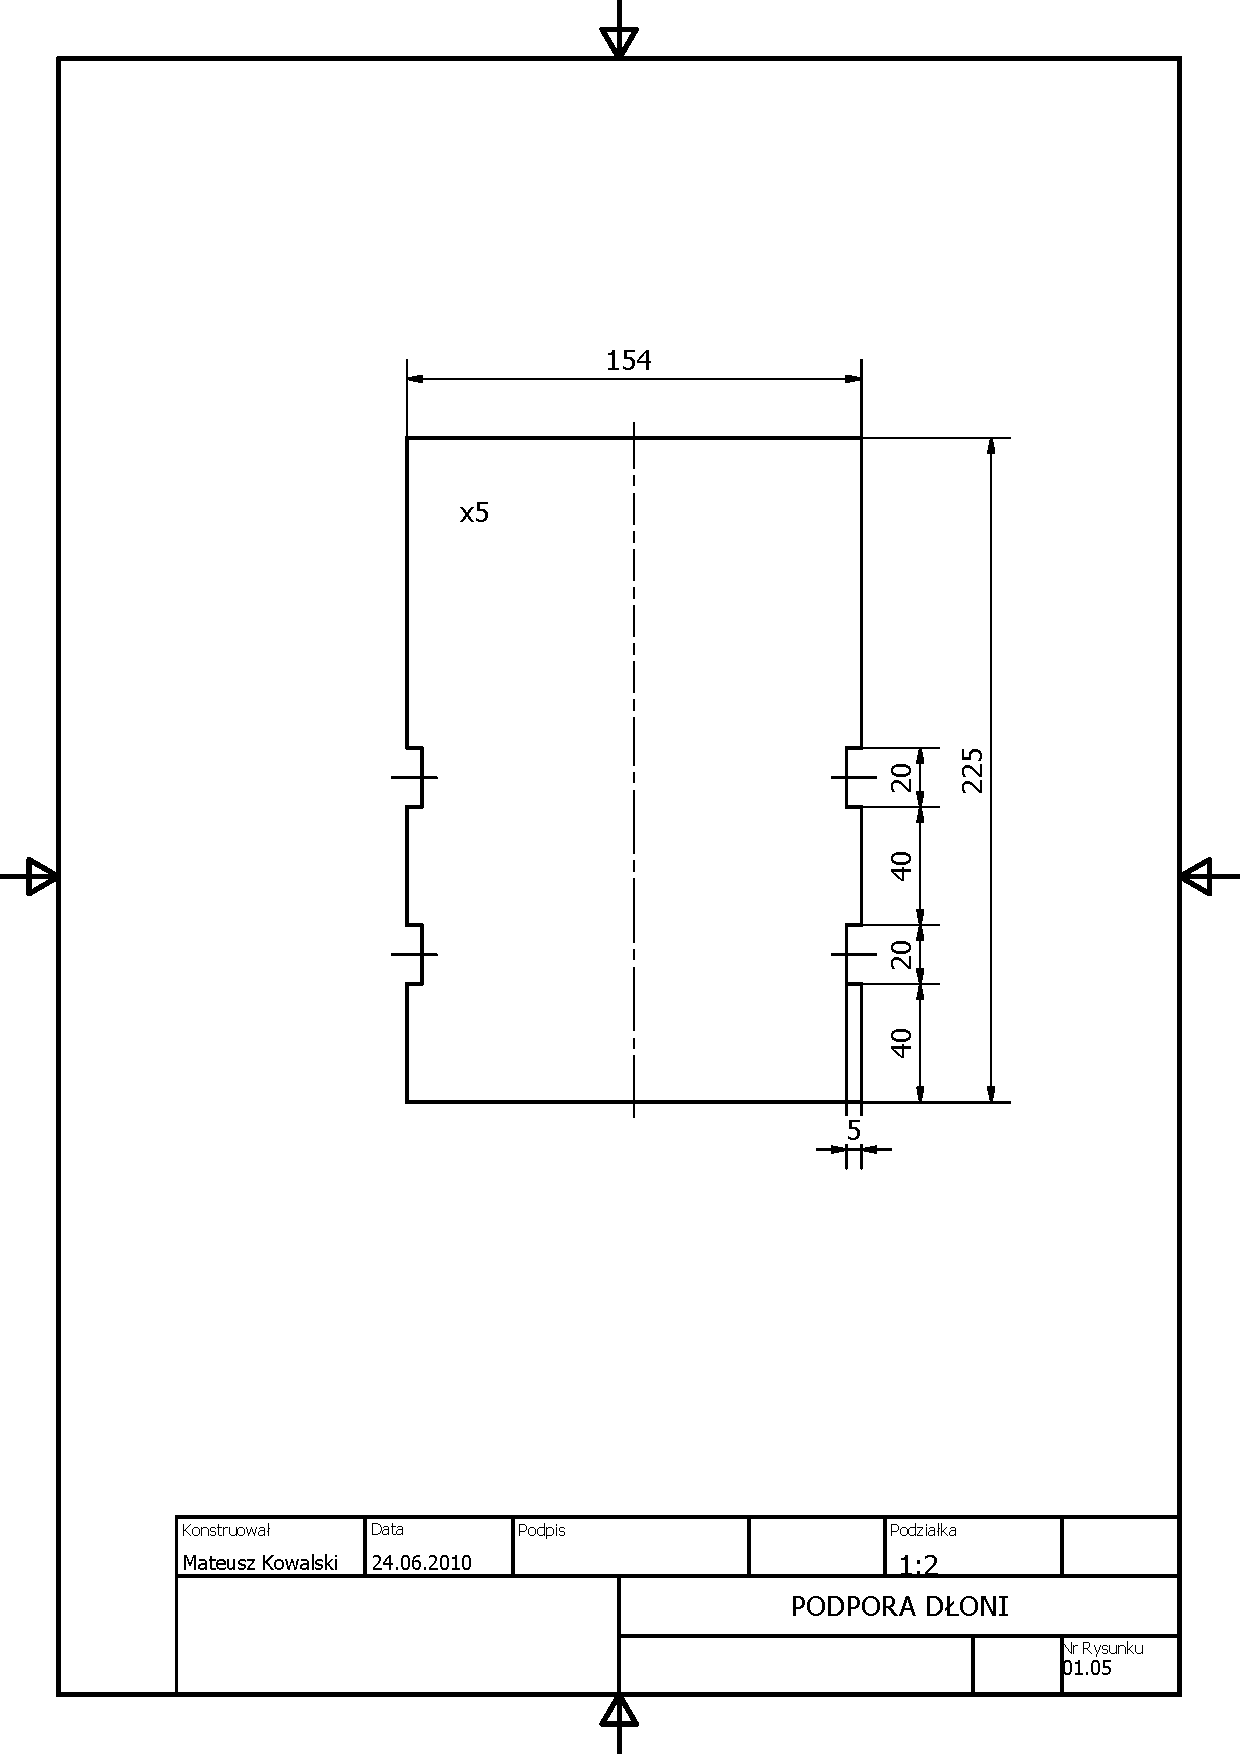
\includepdf{figures/podporadloni.pdf}


\cleardoublepage
\listoftables \cleardoublepage %lista tabel na osobnej stronie
\listoffigures \cleardoublepage %lista rysunków na osobnej stronie

% Bibliography (books, articles) starts here.
\bibliography{bibliografia}

% Colophon is a place where you should let others know about copyrights etc.
\ppcolophon

\end{document}
